\section{Vergleichsrechnung mit Newton-Euler-Verfahren}

Die Rechnung wird für debugging Ziele und leichtere Simulation (Rechneraufwandweise) nur nach der Simulation passieren. 
Weswegen sollen die Daten aus der Simulation nach MATLAB-Workspace übertragen werden. Für diese Zwecke kann \en{ToWorkscape} MATLAB-Block verwendet werden.
Die Daten in dieser Arbeit werden für jeden Zeitpunkt der Simulation gespeichert.

	\begin{figure}[!htbp]
		\centering
		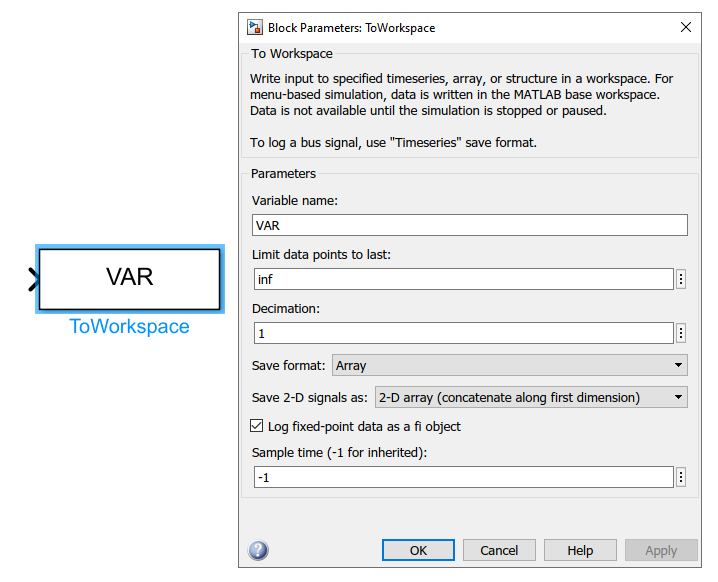
\includegraphics[width=1\linewidth]{grafic/to_workspace_block}
		\caption{ToWorkspace MATLAB-Block}
		\label{fig:simulink_to_workspace}
	\end{figure}

	\subsection{Abschätzung von Massen und Trägheiten. Ermittlung von Rotationsmatzen, p- und s-Vektoren}

Damit die Massen, Trägheiten und s-Vektoren aus der Simulation genommen werden können, in Simulink steht \en{Inertia Sensor} zur Verfügung.
Für die Rotationsmatrizen, p-Vektoren werden \en{Transformation Sensor} zur Verfügung gestellt.
Die Sensoren werden in einem Subsystem eingeschloßen. Linke Port der Subsystem entspricht i. Koortinatensystem. Rechte Port entspricht i+1. Koordinatensystem.

	\begin{figure}[!htbp]
		\centering
		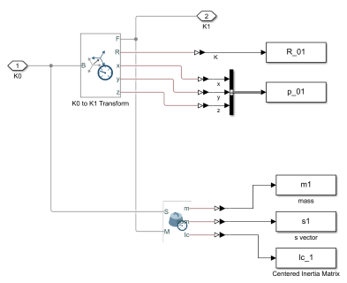
\includegraphics[width=1\linewidth]{grafic/sensor_koordinatensystem}
		\caption{Beispiel des Sensorensubsystems}
		\label{fig:sensoren_subsystem}
	\end{figure}


\subsection{Berechnung mit Newton-Euler-Verfahren}

	\subsubsection{\en{compute_torques_with_newton-euler.m}}

	Dieses Skript wird nach der Simulation ausgeführt (StopFnc Callback in Simulink).
	Es führt manche Manipulationen mit den Daten, damit sie leichter werden zu bearbeiten.

==========================================>>>>>>>>> (language=MATLAB)
	if size(q,1) > size(q,2)
		q = q';
		q_dot = q_dot';
		q_2dot = q_2dot';
		tau_sim = tau_sim';
	end

	sim_steps = length(q(1,:));
	n_joints = length(q(:,1));

	omega = zeros(3, n_joints, sim_steps);
	omega_dot = zeros(3, n_joints, sim_steps);
	v_dot = zeros(3, n_joints, sim_steps);
	vs_dot = zeros(3, n_joints, sim_steps);
	tau = zeros(n_joints, sim_steps);

	% concatenate data from simulation for easier iteration
	R = cat(4, R_01, R_12, R_23, R_34, R_45, R_56);
	p = cat(3, p_01', p_12', p_23', p_34', p_45', p_56');
	s = cat(3, s1', s2', s3', s4', s5', s6');
	Ic = cat(4, Ic_1, Ic_2, Ic_3, Ic_4, Ic_5, Ic_6);
	m = cat(1, m1, m2, m3, m4, m5, m6);
	m = m';

	for i = 1:sim_steps
		[omega(:,:,i), omega_dot(:,:,i), v_dot(:,:,i), vs_dot(:,:,i)] = ...
			compute_kinematics(q(:,i), q_dot(:,i), q_2dot(:,i), R(:,:,i,:), R_W0(:,:,i), p(:,i,:), s(:,i,:));
		tau(:,i) = compute_forces_and_torques(omega(:,:,i), omega_dot(:,:,i), vs_dot(:,:,i), m, Ic(:,:,i,:), p(:,i,:), s(:,i,:), R(:,:,i,:));
	end

	ts = timeseries(tau, tout, 'Name', 'tau');
<<<<<<<<<==========================================

	\subsubsection{\en{function compute_kinematics()}}

Diese Funktion repräsentiert ersten Schritt in Newton-Euler-Verfahren - "kinematische Berechnung".

	\begin{figure}[!htbp]
		\centering
		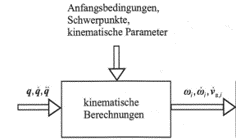
\includegraphics[width=1\linewidth]{grafic/compute_kinematics_diagramm}
		\caption{Beispiel des Sensorensubsystems, Quelle: Roboterdynamik, Vorlesung 11, HHN}
		\label{fig:sensoren_subsystem}
	\end{figure}

Die Funktion berechnet die Werte der Geschwindigkeit und Beschleunigungen für K1 mit Anfangsbedingungen. 

	\begin{figure}[!htbp]
		\centering
		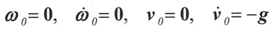
\includegraphics[width=1\linewidth]{grafic/anfangsbedingungen}
		\caption{Anfangsbedingungen kinematischer Berechnung, Quelle: Roboterdynamik, Vorlesung 11, HHN}
		\label{fig:anfangsbedingungen}
	\end{figure}


Dann berechtet sie die Werte von Geschwindigkeiten und Bescheunigungen von K2 bis K6 iterativ.

==========================================>>>>>>>>> (language=MATLAB)
	function [omega, omega_dot, v_dot, vs_dot] = compute_kinematics(q, q_dot, q_2dot, R, R_W0, p, s)
		z = [0 0 1]';
		n_joints = length(q);

		%Anfangsbedingungen
		omega = zeros(3, 6);
		omega(:,1) = q_dot(1)*z;
		
		omega_dot = zeros(3, 6);
		omega_dot(:,1) = q_2dot(1)*z;
		
		
		% Beschluenigung des KSs.
		v_dot(:,1) = inv(R(:,:,1,1)) * (inv(R_W0) * [0 -9.81 0]') + ...
			cross(omega_dot(:, 1), p(:,1,1)) + ...
			cross(omega(:,1), cross(omega(:,1), p(:,1,1))); 

		% Beschleunigung des Schwerpunkts.	
		vs_dot(:,1) = v_dot(:,1) + cross(omega_dot(:, 1), s(:, 1, 1)) + ...
			cross(omega(:, 1), cross(omega(:,1), s(:, 1, 1))); 
		
		for i = 1:n_joints-1
			invR = inv(R(:,:,1,i));

			omega(:,i+1) = invR * (omega(:,i) + q_dot(i+1)*z);
			omega_dot(:,i+1) = invR * (omega_dot(:,i) + ...
				(z * q_2dot(i+1) + cross(omega(:,i), q_dot(i+1) * z)));

			v_dot(:, i+1) = invR * v_dot(:,i) + ...
				cross(omega_dot(:, i+1), p(:,1,i+1)) + ...
				cross(omega(:,i+1), cross(omega(:,i+1), p(:,1,i+1)));
			vs_dot(:,i+1) = v_dot(:,i+1) + ...
				cross(omega_dot(:, i+1), s(:, 1, i+1)) + ...
				cross(omega(:, i+1), cross(omega(:,i+1), s(:, 1, i+1)));
		end
	end
<<<<<<<<<==========================================


	Die Gleichungen, die in der Funktion berechnet werden.

	\begin{figure}[!htbp]
		\centering
		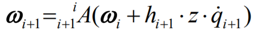
\includegraphics[width=1\linewidth]{grafic/omega_gleichung}
		\caption{Winkelgeschwindigkeit Gleichung, Quelle: Roboterdynamik, Vorlesung 11, HHN}
		\label{fig:omega_gleichung}
	\end{figure}

	\begin{figure}[!htbp]
		\centering
		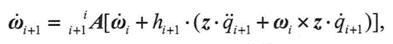
\includegraphics[width=1\linewidth]{grafic/omega_dot_gleichung}
		\caption{Winkelbeschleunigung Gleichung, Quelle: Roboterdynamik, Vorlesung 11, HHN}
		\label{fig:omega_dot_gleichung}
	\end{figure}

	\begin{figure}[!htbp]
		\centering
		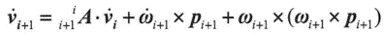
\includegraphics[width=1\linewidth]{grafic/v_dot_gleichung}
		\caption{Geschwindigkeit des KSs Gleichung, Quelle: Roboterdynamik, Vorlesung 11, HHN}
		\label{fig:v_dot_gleichung}
	\end{figure}

	\begin{figure}[!htbp]
		\centering
		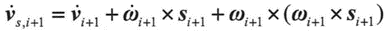
\includegraphics[width=1\linewidth]{grafic/vs_dot_gleichung}
		\caption{Geschwindigkeit des Schwerpunkts Gleichung, Quelle: Roboterdynamik, Vorlesung 11, HHN}
		\label{fig:vs_dot_gleichung}
	\end{figure}


\subsubsection{\en{function compute_forces_and_torques()}}

Diese Funktion repräsentiert zweiten Schritt in Newton-Euler-Verfahren - "Berechnungen der Kräfte und Drehmomente".

	\begin{figure}[!htbp]
		\centering
		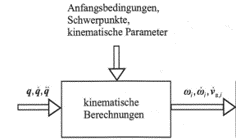
\includegraphics[width=1\linewidth]{grafic/compute_kinematics_diagramm}
		\caption{Berechnungen der Kräfte und Drehmomente, Quelle: Roboterdynamik, Vorlesung 11, HHN}
		\label{fig:sensoren_subsystem}
	\end{figure}

===============================================>>>>>>>(language=MATLAB)

function [tau] = compute_forces_and_torques(omega, omega_dot, vs_dot, m, Ic, p, s, R)
	z = [0 0 1]';
	n_joints = length(omega(1,:));
	% auf n_joints+1 stehen Anfangskräfte und -drehmomente.
	f = zeros(3, n_joints+1);
	n = zeros(3, n_joints+1);
	tau = zeros(1, n_joints);
	R(:,:,1,7) = eye(3,3);

	for i = n_joints:-1:1
		F(:,i) = m(i) * vs_dot(:, i);
		f(:,i) = R(:,:,1,i+1) * f(:,i+1) + F(:,i);
		N(:,i) = Ic(:,:,1,i) * omega_dot(:,i) + cross(omega(:,i), Ic(:,:,1,i) * omega(:,i));
		n(:,i) = n(:,i+1) + cross(p(:,1,i)+s(:,i), F(:,i)) + cross(p(:,i), f(:,i+1)) + N(:,i);
		tau(i) = n(:,i)' * inv(R(:,:,1,i)) * z;
	end

end

<<<<<<<<==============================================

Die Gleichungen, die in der Funktion berechnet werden.

	\begin{figure}[!htbp]
		\centering
		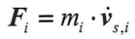
\includegraphics[width=1\linewidth]{grafic/Fi_gleichung}
		\caption{Kraft an einem Schwerpunkt Gleichung, Quelle: Roboterdynamik, Vorlesung 11, HHN}
		\label{fig:Fi_gleichung}
	\end{figure}

	\begin{figure}[!htbp]
		\centering
		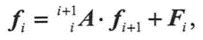
\includegraphics[width=1\linewidth]{grafic/klein_fi_gleichung}
		\caption{Gelenkkraft Gleichung, Quelle: Roboterdynamik, Vorlesung 11, HHN}
		\label{fig:klein_fi_gleichung}
	\end{figure}

	\begin{figure}[!htbp]
		\centering
		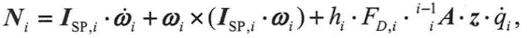
\includegraphics[width=1\linewidth]{grafic/gross_n_gleichung}
		\caption{Wirkenden Drehmonent Gleichung, Quelle: Roboterdynamik, Vorlesung 11, HHN}
		\label{fig:gross_n_gleichung}
	\end{figure}

	\begin{figure}[!htbp]
		\centering
		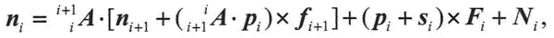
\includegraphics[width=1\linewidth]{grafic/klein_n_gleichung}
		\caption{Drehmomente in dem Gelenk Gleichung, Quelle: Roboterdynamik, Vorlesung 11, HHN}
		\label{fig:klein_n_gleichung}
	\end{figure}

	\begin{figure}[!htbp]
		\centering
		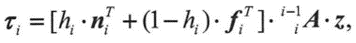
\includegraphics[width=1\linewidth]{grafic/tau_gleichung}
		\caption{Drehmomente in dem Gelenk Gleichung, Quelle: Roboterdynamik, Vorlesung 11, HHN}
		\label{fig:tau_gleichung}
	\end{figure}





